\section{方法}
  \subsection{使用機器・開発環境}
    使用するヘッドマウントディスプレイ(HMD)はMeta Quest Proを採用する.
    このHMDは高解像度,広視野角に加えて優れた空間認識機能を備えているため,
    被験者に高度な没入体験を提供することができる.
    \\\indent
    開発環境はUnityエンジンを使用し,
    可能な限り実際のパズル体験に近づける.
    \\\indent

  \subsection{VR環境の構築}
  %======================================================================================
    ルービックキューブを解くことが目的であるため,
    環境は机のみが配置されている簡素な部屋をモデルとする.
    \\\indent
    一般的な3×3×3のルービックキューブは組み合わせが約430京通りあり,
    覚える手順も最低でも6から8個が必要である.
    一方で2×2×2のものは組み合わせが約370万通り,
    覚える手順も2から3個と少ない.
    揃えることがより容易である
    2×2×2のルービックキューブを採用する(図\ref{cube}).
    解法教示の表示などはおこなわない.
  %======================================================================================
    \begin{figure}[h]
      \begin{center}
        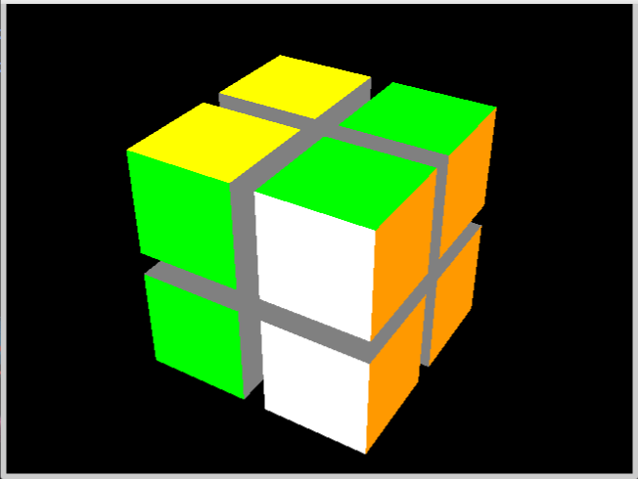
\includegraphics[width=50mm]{./images/cube.png}
        \caption{使用するルービックキューブ}\label{cube}
      \end{center}
    \end{figure}
  %======================================================================================
